% !TEX root = ../thesis-sample.tex

\chapter{Leveraging the household sector’s ideas} \label{chap:ECAST}

\section{Introduction}
A new paradigm of innovation recognizes the efforts of individuals within the general public, or “household sector” (von Hippel, 2017), who feel strongly enough about a problem to create and share their ideas for free. Scholars theorize that this process is highly personal or “local” (von Hippel, 2017, 2005). Individuals view—or formulate (Lüthje et al., 2005; Shah and Tripsas, 2007)—the problem through their perceptions and experiences. Their choice of knowledge to apply is also informed by their background (Franke et al., 2013; Jeppesen and Lakhani, 2010). The resulting combinations of formulations and knowledge can be valuable to those who cannot draw on the same material (Afuah and Tucci, 2012; Franke et al., 2013; Prahalad, 2004)—they are “distant” from it. Additionally, these individuals represent a significant portion of the general public (de Jong, 2016; von Hippel et al., 2012, 2011), contributing across a wide range of domains like baby products (Poetz and Schreier, 2012), mountain bikes (Lüthje et al., 2005), and medical devices (Lettl et al., 2009; von Hippel, 2017). 

Despite the household sector’s potential for capability and capacity, organizations have struggled to leverage them alongside their internal efforts. In fact, organizations judge most contributions from the innovative public to be of little value. For example, BP’s call for ideas after the Deepwater Horizon oil spill in the Gulf of Mexico received 120,000 contributions (Gulf Coast Ecosystem Restoration Council, 2010) to seal the well or clean up the affected waterways (Goldenberg, 2011). According to BP, however, the public’s effort “yielded very little in terms of results” (Goldenberg, 2011) and did not translate into a solution that went “all the way” (Alexy et al., 2012, p. 117) to implementation. These scenarios highlight the current inability to bridge the public-organization gap successfully. Organizations can prompt a large amount of free effort from the public. However, their efforts are wasted if the problem is mismatched for the public’s strengths, or their resulting contributions are not—or cannot—be translated into the organization’s context.    

This work is an attempt to bridge that gap. The literature has theorized that the public’s local knowledge (Afuah and Tucci, 2012; Franke et al., 2013; Jeppesen and Lakhani, 2010) and local formulation (Lüthje et al., 2005) of the problem are drivers for quality. Scholars have also explored how a contribution that is distant or lacks enough depth can be misjudged (di Gangi et al., 2010; di Gangi and Wasko, 2009; Piezunka and Dahlander, 2014), even if it solves the problem. In this paper, we studied how the constructs of local knowledge, local formulation, and depth influence the substance of the public’s contributions, based on their impact within the focal organization. 

To answer this question, we selected a setting where the public’s contributions to a problem were meaningful to the focal organization. National Aeronautics and Space Administration (NASA)’s Asteroid Initiative was a program tasked with consolidating asteroid activities in the agency, as well as engaging with individuals and entities outside of the NASA’s established planetary defense community. We observed this program and its events across several years. Here, our data captured NASA’s change in perception of public contributions over time. Our data also captured the public’s solving processes and contributions to a mission design problem in a citizen forum—an event that played a crucial role in the perception change. Our analysis linked these two: we connected the public’s solving dynamics to this change in perception by unpacking how and when the public created contributions that were deemed substantive by NASA.

While current theory implies direct links between the public’s problem-solving strengths and the substance of their contribution, we find only partially support for these relationships. As anticipated by theory, an individual’s use of their local knowledge correlated directly to the substance of their contribution. In contrast, the impact of an individual’s local formulation was more nuanced. Local formulation—reformulating the NASA problem in their own terms—increased the substance of their contribution because it increased the depth of said contribution. That is, the relationship between substance and formulation was fully mediated by depth of the contribution. Lastly, the interaction of local knowledge and local formulation consistently reduced the likelihood of a substantive contribution. 

Our findings contribute to understanding how organizations can leverage the public’s problem-solving efforts alongside their own (Chatterji and Fabrizio, 2011; Goucher-Lambert and Cagan, 2019; Lifshitz-Assaf, 2018; Lüthje et al., 2005; Szajnfarber and Vrolijk, 2018). We unpacked how the public created their most valuable contributions (Acar, 2019; Stock et al., 2016) to a problem that the focal organization considered important. We also studied the interaction of problem-solving constructs that are rarely examined at the same time (Gralla et al., 2016). More broadly, this work is an existence proof that the free innovation paradigm can be directed.

We organized this paper as follows: first, we review the literature on local knowledge, local formulation, and depth of contributions. Next, we describe our setting, the data stemming from it, as well as the methods used in our analysis. Then, we present our results, and discuss these in the context of our setting and the existing literature. We conclude by explaining the limitations of the study, as well as outlining potential areas of future work. 



\section{General Usage}
The way to invoke usage of this template is to put
\begin{verbatim}
\documentclass{thesis-gwu.cls}
\end{verbatim}
at the beginning of your preamble.  
This can also work if the \texttt{thesis-gwu.cls} file is not in the same directory as your \texttt{.tex} file.  
To do so, just give the relative path.
\begin{verbatim}
\documentclass{./tex/thesis-gwu.cls}
\end{verbatim}

Much like a usual article or report in \LaTeX, the user specifies the primary information about the document in the preamble with commands like
\begin{verbatim}
\author{Shankar Kulumani}
\chair{Taeyoung Lee}
\end{verbatim}
At the beginning of the document, the title page will automatically be created and inserted at the beginning of the document.  
If you forget to declare any of the required fields, it will generate a title page with a message such as ``Insert an author!''

However, the template does a lot more in the preamble than just create a title page.  
The preamble (that is, whatever comes before \texttt{begin\{document\}} in the primary \texttt{.tex} file) is also the place for the user to specify a dedication, any acknowledgments, a foreword, \textit{etc.}  
This is done in a manner very similar manner to declaring the author, title, and so on. Suppose that someone wants to have a simple dedication ``To Mom'', the following command is all that is needed.
\begin{verbatim}
\dedication{To Mom}
\end{verbatim}
This will cause the document to have a dedication page with the
corresponding text.  
If the \texttt{dedication} command is not present, there will not be a dedication page.  
All the work of either having or not having a dedication has been compressed into a single command!
Things other than simple text \emph{are} allowed in the dedication, so feel free to put equations or whatever inside there.  
There are a few more commands that can be used to customize the appearance of the dedication page, and also for the other preamble text pages, but that is left to~\cref{ssec:dedication}.

\section{Front Matter}
The \LaTeX term ``frontmatter'' refers to all of the pages that occur before the beginning of the first chapter.  
It is usually made clear to the reader because the pages in the front matter are numbered with lower-case Roman numerals instead of Arabic numerals.

The present template, \texttt{thesis-gwu.cls} attempts to remove as much work associated with the front matter as possible.  
The template inserts all of the front matter pages automatically, so that there is
not even a need to use a command like \verb+\maketitle+.  
The first thing after \verb+\begin{document}+ should be the start of the first
chapter.

\subsection{Identifiers}
The template is not able to read minds, of course, so there needs to be some way of inputting the relevant information.  
This section covers how to specify the author, title, and so on.  
For the most part, this works just like any other \LaTeX~document, but a dissertation has a few more identifiers than most documents (How many books or reports have a
committee?).  
So there are a few extra commands provided by this template, and they work \emph{almost} exactly like the standard commands.

\begin{table}
 \caption{ \label{tab:identifiers}
  List of all identifier commands}
 \centering
 \small
 \begin{tabular}{l @{\hspace{16pt}} l @{\hspace{16pt}} p{6cm}}
  \hline \hline
  \textsc{Item} & \textsc{Usage} & \textsc{Comment} \\
  \hline
  Author      & \verb|\author{...}|
   & Works as in standard \LaTeX \\
  Chair       & \verb|\chair{...}|
   & Name of chair \emph{without} any title or affiliation.  This
     appears only on the abstract page, and only if there is no
     co-chair. \\
  Co-chair    & \verb|\cochair{...}|
   & Names of all co-chairs \emph{without} any titles or
     affiliations.  This appears only on the abstract page.  Note
     that by convention, it is not chair \emph{and} co-chair, but
     just two co-chairs. \\
  Committee   & \verb|\committee{...}|
   & Formatted names of committee members \emph{with} the
     appropriate titles and university names.  This will appear
     only on the title page. \\
  Department  & \verb|\department{...}|
   & Title of department of student \\
  Title       & \verb|\title{...}|
   & Works as in standard \LaTeX \\
  Year        & \verb|\year=2012|
   & Year that dissertation will be \emph{completed} \\
  \hline \hline
 \end{tabular}
\end{table}

A full list of the identifiers is given in Table \cref{tab:identifiers}. 
You're free to adjust/delete these commands as desired.



\subsection{Frontispiece and Copyright}

By default, the template assumes that there should be a copyright page, and the copyright holder is the author.  
To prevent the copyright page from appearing, use the command \verb|\hidecopyright|.  
To assign the copyright to someone other than the author, use the following command.
\begin{verbatim}
\copyrightholder{Someone Else}
\end{verbatim}


\subsection{Text Pages}  \label{ssec:dedication}
The handling of the first few pages after the title page is one of the best features of this template.  
The pages that occur between the copyright page and the abstract page all consist of short pieces of text that are usually a single paragraph.  
The text for each of these pages is set up using a command of the same name.
Generally, only one of the front matter pages is used. 
\begin{verbatim}
\foreword{This is going to be the best dissertation ever.}
\end{verbatim}
Usually the contents of each of these pages will be longer than a single sentence, and thus it should be noted that each of these commands allows most types of \LaTeX~input.  
For example, the following is perfectly acceptable input--at least as far as the template is concerned.
\begin{verbatim}
\foreword{This is going to be the \emph{best}. \\
 \begin{center} Really, really. \end{center}}
\end{verbatim}

As I mentioned before, a given page will appear in the document if and only if the corresponding command is used.  
The order in which the pages appear does not depend on the order the commands are used in the preamble.  
You can also prevent the pages from appearing by using commands like \verb|\hideforeword|.

The style of each page can also be set by the user.  
By default, each page will appear with a bold, italic heading corresponding to the name
of the page.  
However, there are five other formats, which can be controlled using an optional argument.  
For example, the following command creates a dedication page with no heading (\textit{i.e.}~it does not say ``Dedication'' on the page) but with lines above and below the dedication text.
\begin{verbatim}
\dedication[4]{To Mom}
\end{verbatim}
A complete list of the available styles is given in \cref{tab:fronstyle}.  
The style of each page can be set independently, but it is also possible to change which style is used by default.
\begin{verbatim}
\frontpagestyle{6}
\end{verbatim}
This would make all of the commands that were called without optional
inputs to create pages using style 6.  

\begin{table}
 \caption{ \label{tab:fronstyle}
  List of styles for frontmatter text pages}
 \centering
 \begin{tabular}{c @{\hspace{16pt}} p{8cm}}
  \hline \hline
  \textsc{Style} & \textsc{Description} \\
  \hline
  1 & Justified text with no header or lines \\
  2 & Justified text with bold italic header and no lines \\
  3 & Justified text, capitalized header, no lines \\
  4 & Justified text with lines and no header \\
  5 & Justified text with bold italic header and lines \\
  6 & Justified text with capitalized header and lines \\
  other & Centered text with no header or lines \\
  \hline \hline
 \end{tabular}
\end{table}



\subsection{Lists of Things}   \label{ssec:lists}
Suffice it to say that this template handles the Table of Contents appropriately, but this section is also meant to address the List of Figures, List of Tables, \textit{etc}.  According to the guidelines, a corresponding list must appear if there is more than one figure, table, map, program, illustration, or appendix.  
The template assumes that the dissertation will contain at least two figures and tables.
If, for example, there is only one figure,
\begin{verbatim}
\hidelistoffigures
\end{verbatim}
must be put in the preamble.
There are similar commands to hide/show all of the front matter pages.
These can be used at will as desired.

\subsection{Glossary of Terms}\label{ssec:glossary}
Here is an example.
\Gls{linux} is a computer operating system, and its completely free and open.

A \gls{matrix}, denoted \gls{M}.
Lots of \glspl{matrix}.
\Glspl{matrix} are a rectangular array of quantities.
No indexing, linking, or formatting: \glsentrytext{matrix}.
The identity \gls{matrix}['s] diagonal consists of ones.

First use: \gls{filo}.
Next use: \gls{filo}.
Full form: \acrfull{filo}.


\subsection{Acronymns and Symbols}\label{ssec:acronymns}
The other type of list that can occur is for abbreviations of various types.  
This is a somewhat convenient feature, particularly there are a lot of acronyms in the dissertation.  
This template utilizes the \texttt{acronym} or \texttt{glossaries} packages, but eventually I would like to migrate to the use of \texttt{glossaries} which is continuing to be supported and deprecate the use of \texttt{acronym}, for now both are supported. 

\subsubsection{\texttt{acronymn} usage - try to avoid using this as it's not the best}
In the preamble put a command like the following.
\begin{verbatim}
\abbreviations{
 \acro{CFD}{Computational Fluid Dynamics}
 \acro{LOA}{List of Abbreviations}
 \acro{H2O}[$\mathrm{H_2O}$]{water}}
\end{verbatim}
This will define a bunch of abbreviations that can be used.  
When you want to use one of the acronyms within the text, simply use the \verb|\ac| command to refer to the abbreviation you want.  
This will automatically spell out what the abbreviation stands for on the first use and only print out the abbreviation on subsequent uses.  

\subsubsection{\texttt{glossaries} usage - much improved and more powerful}
In addition, you can utilize the much more powerful \texttt{glossaries} package.
You can define symbols, acronymns, or full glossary entries as desired.
Each acronymn is defined using the following:
\begin{verbatim}
\newacronym{crtb}{CRTBP}{Circular Restricted Three Body Problem}
\end{verbatim}
Here we can  use an acronym, such as \gls{crtbp}.
Or display the full name, \gls{crtbp}.

\section{Float environments}
There are many possible float enviornments, and this section will serve as an introduction and demonstration of some of them.
In addition, it offers the ability to ensure that this template actually follows the guidelines.

\subsection{Figures}\label{ssec:figures}

Here is a figure as shown in~\cref{fig:picard}.
Notice how we're using the fancy referencing offered by the \verb+cleveref+ package. 
Instead of using the normal~\verb+\ref+ command we instead use~\verb+\cref+. 
The magic of \LaTeX automatically figures out that the previous reference points to a figure while~\cref{ssec:figures} points to a section.

\begin{figure}
    \centering
    \includegraphics[width=0.5\textwidth]{figures/picard_yes.jpg}

    \caption[Damage report!]{Glad to have a thesis class\label{fig:picard}}
\end{figure}

Here's another figure that demonstrates the use of \texttt{tikz} and the externalization library.
\begin{figure}
    \centering
    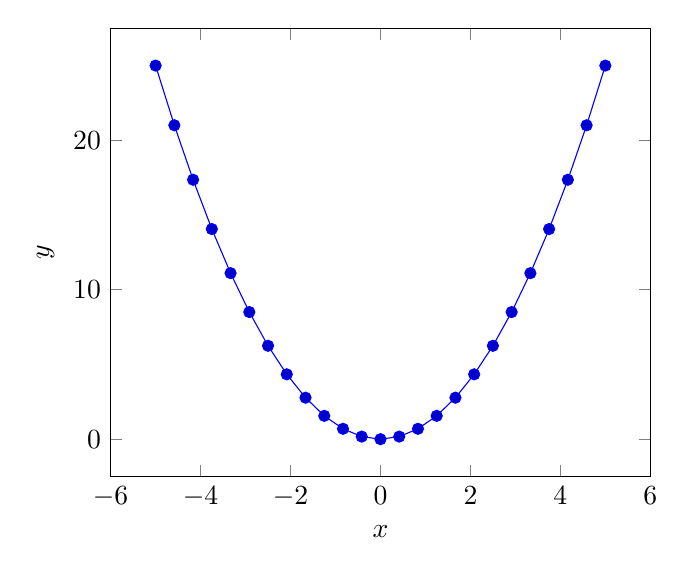
\begin{tikzpicture}
        \begin{axis}[
            xlabel={$x$},
            ylabel={$y$},
            ]
            \addplot {x^2};
        \end{axis}
    \end{tikzpicture}
    \caption{Externajhjhjhjjhi\label{fig:tikz}}
\end{figure}

\subsection{Tables}\label{ssec:tables}

Here's a table in~\cref{tab:table}

\begin{table}
\begin{center}
    \begin{tabular}{ | l | l | l | p{5cm} |}
    \hline
    Day & Min Temp & Max Temp & Summary \\ \hline
    Monday & 11C & 22C & A clear day with lots of sunshine.  
    However, the strong breeze will bring down the temperatures. \\ \hline
    Tuesday & 9C & 19C & Cloudy with rain, across many northern regions. Clear spells 
    across most of Scotland and Northern Ireland, 
    but rain reaching the far northwest. \\ \hline
    Wednesday & 10C & 21C & Rain will still linger for the morning. 
    Conditions will improve by early afternoon and continue 
    throughout the evening. \\
    \hline
    \end{tabular}
    \caption[Short caption for table]{Long caption for text \label{tab:table}}
    \end{center}
\end{table}

\section{References and Citation}
Finally, we'll add a subfigure to demonstrate it's proper use. 
Many people use the package~\verb+subfigure+ but this is in fact, quite wrong. 
To begin, the~\verb+subfigure+ package has been deprecated, which one can check by going to \url{https://www.ctan.org/pkg/subfigure}{CTAN}.
Instead, everyone should be using~\verb+subcaption+, just as this class file is already doing.
Here, in~\cref{fig:xkcd}, we see two subfigures encapsulated in a larger figure environment.
Luckily, with our fancy referencing we have access to both~\cref{fig:ext,fig:ksp} using the same commands.
The key thing to note from~\cref{fig:ext} is that trustworthiness reaches a maximum for those using~\verb+.tex+.


\subsection{References}

Lots of famous people tend to write famous papers~\cite{newton1999}. 
Were they famous because or in-spite of their papers?
Regardless, they're famous now and we all should read them.
Certain people are so famous and do such great work that they invent a whole new field of study with a single paper~\cite{kalman1960,shannon1949}

\section{Math}

Here are some nice equations~\cref{prob_def,prob_def_constrained}
\begin{align}
\label{prob_def}
&\min_{s\subset W}\ J(s) = \sum_{i=1}^{l-1} H(s_j, s_{j+1}) \\
&\max_{s\subset W}\ P_{tr}(s) = \prod_{i=1}^{l-1} P_{tr}(s_j, s_{j+1}) \nonumber
\end{align}

Here's another equation.
\begin{align}
\label{prob_def_constrained}
&\min_{s\subset W}\ J(s) = \sum_{i=1}^{l-1} H(s_j, s_{j+1}) \\
&\text{subject to} \ P_{tr}(s)>\epsilon_{tr} \nonumber
\end{align}






